\section{Porkchop plots analysis}

This section presents the results computed for a direct orbit transfer between
Earth and the two interstellar objects. The analysis is performed by solving the
Lambert's problem under the Keplerian assumption.

The algorithm used is the one devised by \cite{izzo2015}, as it is proven to be
more accurate and faster than other classical algorithms \cite{martinez2021}.
The ephemerides for 1I/'Omuaumua and 2I/Borisov are obtained from JPL Horizons
API service. These are propagated under the two-body assumption to simplify the
analysis. Propagation starts on January 1, 2016 and ends on January 1, 2035.

\subsection{Characteristic energy anslysis}

Porkchop plots for 'Oumuaumua and Borisov are shown in figure
\ref{fig:oumuamua-direct-transfer-porkchop} and figure
\ref{fig:borisov-direct-transfer-porkchop}. The limits for the characteristic
energy range between 0 and 12000 km$^2$/s$^2$. Isolines for the time of flight
are also included in these plots.

\newpage
\begin{figure}[H]
  \centering
  \includegraphics[width=\textwidth]{static/oumuamua/direct-transfer-porkchop.png}
  \caption{Launch energy porkchop plot for 1I/'Oumuamua.}
  \label{fig:oumuamua-direct-transfer-porkchop}
\end{figure}
\begin{figure}[H]
  \centering
  \includegraphics[width=\textwidth]{static/borisov/direct-transfer-porkchop.png}
  \caption{Launch energy porkchop plot for 2I/Borisov.}
  \label{fig:borisov-direct-transfer-porkchop}
\end{figure}
\newpage

The contour maps show a periodic pattern, with a minimum energy transfer
corridor every year. This year corresponds to a more favorable position of the
Earth with respect to the interstellar object.

The most energy consuming transfers are located in the lower right corner of the
plot. This area corresponds to a shorter time of flight (4 years). The shorter
the time of flight, the greater the launch velocity and the energy required to
perform the transfer. On the other hand, the upper left corner corresponds to a
longer time of flight (17 years), with lower energy requirements.

It is worh noting that the energy required to reach 'Oumuamua is slightly lower
than the energy required to reach Borisov. This is due to the higher velocity of
this object, since 'Oumuamua is travelling at $26.0$ km/s whereas Borisov does
at $32.2$ km/s.

Finally, both porkchops show a similar contour map. This is due to the long
distance exhibited by the two interlopers in the future positions depicted in
the porkchop plot. The short-time transfer scenarios show differences between
'Oumuamua and Borisov, but the long-time transfer scenarios show similar values.

\subsection{Arrival velocity analysis}

Figures \ref{fig:oumuamua-direct-transfer-porkchop-avl} and
\ref{fig:borisov-direct-transfer-porkchop-avl} show the isolines for the excess
arrival velocity. Values up to $24$ km/s are represented. Higher values may be
represented but they are not shown in the plots for graphic convenience.

The values are extraordinary high. Even if with a targeting mission (no second
impulse), the available observation time and coma samples capture would be
minimum. The direct rendezvous scenario seems unfeasible for nowadays
technology.

For 'Oumuamua, launch dates after 2022 lead to an excess arrival velocity
greater than $10$ km/s. For Borisov, any launch date after 2023 leads to the same
situation.

It is worth noting that the optimum dates for a lower closer to the discovery of
the interlopers. If a ready-to-launch mission would have been available, a quick
launch may have lead to a close targeting with these interplanetary objects.

\newpage
\begin{figure}[H]
  \centering
  \includegraphics[width=\textwidth]{static/oumuamua/direct-transfer-porkchop-avl.png}
  \caption{Launch energy porkchop plot for 1I/'Oumuamua showing the isolines for
        excess arrival velocity. Compared to 2I/Borisov, a rendezvous with
        'Oumuamua leads to more excess arrival velocity for the time of flight.}
  \label{fig:oumuamua-direct-transfer-porkchop-avl}
\end{figure}
\begin{figure}[H]
  \centering
  \includegraphics[width=\textwidth]{static/borisov/direct-transfer-porkchop-avl.png}
  \caption{Launch energy porkchop plot for 2I/Borisov showing the isoliens for
        excess arrival velocity. The shorter the flight of time, the greater the
        excess arrival velocity. Values are minimized for a transfer close to
        the discovery of the object.}
  \label{fig:borisov-direct-transfer-porkchop-avl}
\end{figure}
\newpage
